% Intended LaTeX compiler: pdflatex
\documentclass{scrartcl}
    \usepackage{amsmath, amssymb, bm}
		\usepackage[utf8]{inputenc}
		\usepackage[dvipdfmx]{graphicx}
		\usepackage[dvipdfmx]{color}
		\usepackage[backend=biber,bibencoding=utf8]{biblatex}
		\usepackage{url}
		\usepackage{indentfirst}
		\usepackage[normalem]{ulem}
		\usepackage{longtable}
		\usepackage{minted}
		\usepackage{fancyvrb}
    \usepackage[dvipdfmx,colorlinks=false,pdfborder={0 0 0}]{hyperref}
    \usepackage{pxjahyper}
    \usepackage{caption}
\author{情報科学類3年 江畑 拓哉 (201611350)}
\date{}
\title{ヒューマンインタフェース演習課題2}
\begin{document}

\maketitle
\tableofcontents

\section{実験1 平均反応時間計測}
\label{sec:org1843a15}
\subsection{ヒストグラム}
\label{sec:orga98673c}
\begin{center}
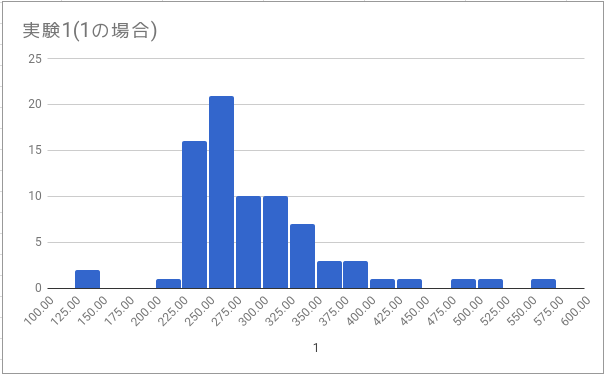
\includegraphics[width=0.5\linewidth]{./1-1.png}
\end{center}
\begin{center}
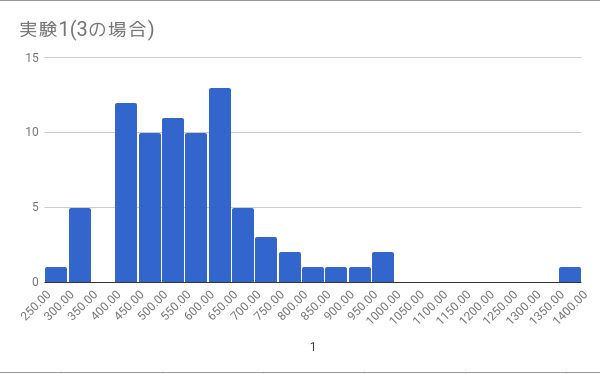
\includegraphics[width=0.5\linewidth]{./1-3.png}
\end{center}
\begin{center}
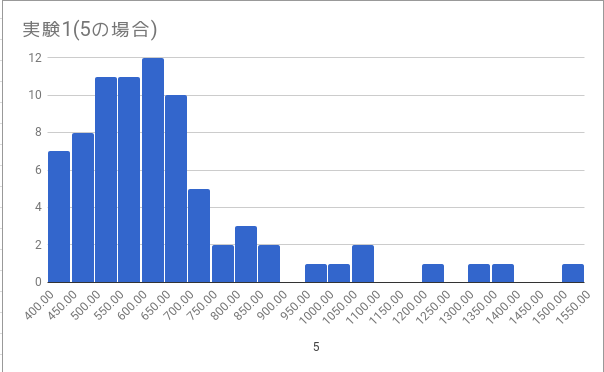
\includegraphics[width=0.5\linewidth]{./1-5.png}
\end{center}
\subsection{平均と最大最小}
\label{sec:orgca670c4}
\begin{center}
\begin{tabular}{rrrr}
\hline
色数 & 平均 & 最大 & 最小\\
\hline
1 & 290 & 551 & 130\\
3 & 567 & 1370 & 270\\
5 & 658 & 1530 & 408\\
\hline
\end{tabular}
\end{center}
\subsection{考察}
\label{sec:org8890805}
 ヒストグラムを見たところ、中央から山のような形になっていることがわかる。正規分布に見えないことはないが、正確にどうかはこのグラフからはサンプル数から判定するのは良くないと考えられる。\\
 またおそらく最大値と最小値はあまり当てにならないと考えられる。なぜなら初回や所謂ぼうっとしたタイミングでボタンを押した場合、勘が当たった場合がこれらに該当すると考えられるからだ。これはグラフの概形の、特に最大値が極端に外れた位置にあることからわかる。\\
\section{実験2 フィッツの実験}
\label{sec:orgaea390e}
\subsection{グラフ}
\label{sec:orgdd0cfdf}
\begin{center}
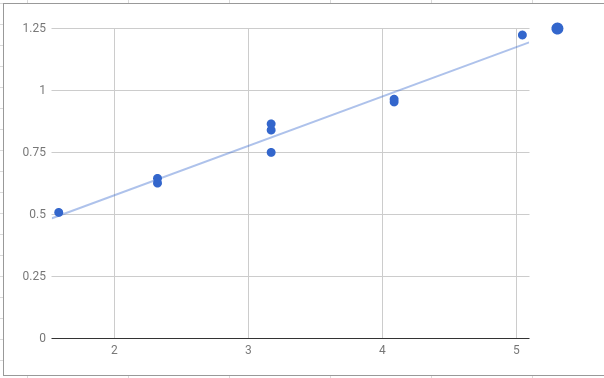
\includegraphics[width=0.8\linewidth]{./2-1.png}
\end{center}
\subsection{考察}
\label{sec:org405b5ac}
 フィッツの法則通り、おおよそ線形になっている事がわかる。\\
 しかし今回は平均値を取っており、実験1のような外れ値を直接目にすることが出来ないためこれらがどの程度影響しているかが正確にはわからなかった。おそらく今回うまく線形に一致したのはどの試行でも同じ程度に外れ値を含んでいたためだと考えられる。\\
\end{document}
